\documentclass[a4paper]{article}
\usepackage{vntex}
\usepackage{a4wide,amssymb,epsfig,latexsym,multicol,array,hhline,fancyhdr}
\usepackage{booktabs}
\usepackage{amsmath}
\usepackage{lastpage}
\usepackage[lined,boxed,commentsnumbered]{algorithm2e}
\usepackage{enumerate}
\usepackage{color}
\usepackage{graphicx}
\usepackage{tabularx, caption}
\usepackage{multirow}
\usepackage[framemethod=tikz]{mdframed}
\usepackage{multicol}
\usepackage{rotating}
\usepackage{graphics}
\usepackage{geometry}
\usepackage{setspace}
\usepackage{epsfig}
\usepackage{tikz}
\usepackage{listings}
\usetikzlibrary{arrows,snakes,backgrounds}
\usepackage{hyperref}
\hypersetup{urlcolor=blue,linkcolor=black,citecolor=black,colorlinks=true}

\newtheorem{theorem}{{\bf Định lý}}
\newtheorem{property}{{\bf Tính chất}}
\newtheorem{proposition}{{\bf Mệnh đề}}
\newtheorem{corollary}[proposition]{{\bf Hệ quả}}
\newtheorem{lemma}[proposition]{{\bf Bổ đề}}

\everymath{\color{blue}}
\setlength{\headheight}{40pt}
\pagestyle{fancy}
\fancyhead{}
\fancyhead[L]{
 \begin{tabular}{rl}
    \begin{picture}(25,15)(0,0)
    \put(0,-8){\includegraphics[width=8mm, height=8mm]{logoITSGUsmall.png}}
   \end{picture}&
	\begin{tabular}{l}
		\textbf{\bf \ttfamily Trường Đại học Sài Gòn}\\
		\textbf{\bf \ttfamily Khoa Công Nghệ Thông Tin}
	\end{tabular}
 \end{tabular}
}
\fancyhead[R]{
	\begin{tabular}{l}
		\tiny \bf \\
		\tiny \bf
	\end{tabular}  }
\fancyfoot{}
\fancyfoot[L]{\scriptsize \ttfamily Bài tập lớn môn Ngôn ngữ lập trình C\# - Niên khóa 2025-2026}
\fancyfoot[R]{\scriptsize \ttfamily Trang {\thepage}/\pageref{LastPage}}
\renewcommand{\headrulewidth}{0.3pt}
\renewcommand{\footrulewidth}{0.3pt}

\setcounter{secnumdepth}{4}
\setcounter{tocdepth}{3}
\makeatletter
\newcounter {subsubsubsection}[subsubsection]
\renewcommand\thesubsubsubsection{\thesubsubsection .\@alph\c@subsubsubsection}
\newcommand\subsubsubsection{\@startsection{subsubsubsection}{4}{\z@}%
                                     {-3.25ex\@plus -1ex \@minus -.2ex}%
                                     {1.5ex \@plus .2ex}%
                                     {\normalfont\normalsize\bfseries}}
\newcommand*\l@subsubsubsection{\@dottedtocline{3}{10.0em}{4.1em}}
\newcommand*{\subsubsubsectionmark}[1]{}
\makeatother

\definecolor{dkgreen}{rgb}{0,0.6,0}
\definecolor{gray}{rgb}{0.5,0.5,0.5}
\definecolor{mauve}{rgb}{0.58,0,0.82}
\definecolor{lightblue}{rgb}{0.9,0.95,1.0}
\definecolor{lightgreen}{rgb}{0.9,1.0,0.9}

\lstset{frame=tb,
	language=CSharp,
	aboveskip=3mm,
	belowskip=3mm,
	showstringspaces=false,
	columns=flexible,
	basicstyle={\small\ttfamily},
	numbers=left,
	numberstyle=\tiny\color{gray},
	keywordstyle=\color{blue},
	commentstyle=\color{dkgreen},
	stringstyle=\color{mauve},
	breaklines=true,
	breakatwhitespace=true,
	tabsize=3,
	stepnumber=1,
	numbersep=5pt,
	firstnumber=1,
	numberfirstline=true
}

\begin{document}

%==========================================================
%                   TRANG BÌA
%==========================================================
\begin{titlepage}
\begin{center}
TRƯỜNG ĐẠI HỌC SÀI GÒN \\
KHOA CÔNG NGHỆ THÔNG TIN
\end{center}
\vspace{1cm}

\begin{figure}[h!]
\begin{center}
\includegraphics[width=3cm]{logoITSGU.png}
\end{center}
\end{figure}

\vspace{1cm}

\begin{center}
\begin{tabular}{c}
	\multicolumn{1}{l}{\textbf{{\Large NGÔN NGỮ LẬP TRÌNH C\#}}}\\
	~~\\
	\hline
	\\
	\multicolumn{1}{l}{\textbf{{\Large Bài tập lớn }}}\\
	\\
	\textbf{{\Huge InteractHub }}\\
	\\
	\textbf{{\large Mạng xã hội tương tác}}\\
	\\
	\hline
\end{tabular}
\end{center}

\vspace{3cm}

\begin{table}[h]
\begin{tabular}{rrl}
\hspace{5 cm} & GVHD: & Từ Lãng Phiêu\\
& SV: & Trần Duy Khương -- 3122410192\\
& & Trương Hữu Nghĩa -- 3122410263 \\
& & Lê Thị Uyên Nhi -- 3122410280 \\
\end{tabular}
\vspace{1.5 cm}
\end{table}

\begin{center}
{\footnotesize TP. HỒ CHÍ MINH, THÁNG 5/2026}
\end{center}
\end{titlepage}

\thispagestyle{empty}
\newpage
\tableofcontents
\newpage

%==========================================================
%  PHẦN 1: GIỚI THIỆU DỰ ÁN
%==========================================================
\section{Giới thiệu dự án}

\subsection{Tổng quan}

\textbf{InteractHub} là một ứng dụng mạng xã hội được xây dựng theo mô hình \textit{full-stack}, lấy cảm hứng từ Facebook, cho phép người dùng đăng bài viết, kết bạn, tương tác qua bình luận và lượt thích, đăng story ngắn, sử dụng hashtag và nhận thông báo theo thời gian thực trong ứng dụng.

Dự án được xây dựng trong môn học \textbf{Ngôn ngữ lập trình C\#}, nhằm vận dụng kiến thức về ASP.NET Core, Entity Framework Core, kiến trúc phân lớp (Layered Architecture), và các kỹ thuật phát triển web hiện đại.

\subsection{Mục tiêu dự án}

\begin{itemize}
    \item Xây dựng hệ thống backend RESTful API hoàn chỉnh sử dụng ASP.NET Core 8.
    \item Thiết kế cơ sở dữ liệu quan hệ với SQL Server thông qua Entity Framework Core.
    \item Xây dựng giao diện người dùng tương tác với React 18 + TypeScript.
    \item Triển khai hệ thống xác thực bảo mật với JWT (JSON Web Token).
    \item Tích hợp CI/CD tự động với GitHub Actions.
    \item Áp dụng các design pattern: Repository Pattern, Dependency Injection, DTO Pattern.
\end{itemize}

\subsection{Công nghệ sử dụng}

\begin{table}[h!]
\centering
\caption{Bảng công nghệ sử dụng trong dự án}
\begin{tabularx}{\textwidth}{|l|l|X|}
\hline
\textbf{Tầng} & \textbf{Công nghệ} & \textbf{Mục đích} \\
\hline
Backend & ASP.NET Core 8 & Framework chính xây dựng Web API \\
\hline
Backend & Entity Framework Core 8 & ORM tương tác cơ sở dữ liệu \\
\hline
Backend & ASP.NET Core Identity & Quản lý người dùng, mã hóa mật khẩu \\
\hline
Backend & JWT Bearer & Xác thực stateless \\
\hline
Backend & SQL Server & Hệ quản trị cơ sở dữ liệu \\
\hline
Backend & xUnit + Moq & Framework kiểm thử đơn vị \\
\hline
Frontend & React 18 + TypeScript & Xây dựng giao diện người dùng \\
\hline
Frontend & Tailwind CSS & Thiết kế giao diện responsive \\
\hline
Frontend & Axios & HTTP Client, tích hợp JWT interceptor \\
\hline
Frontend & React Router v6 & Điều hướng trang và bảo vệ route \\
\hline
Frontend & Vite & Công cụ build nhanh cho frontend \\
\hline
DevOps & GitHub Actions & CI/CD tự động build, test, deploy \\
\hline
DevOps & Azure App Service & Triển khai backend \\
\hline
DevOps & Azure Static Web Apps & Triển khai frontend \\
\hline
\end{tabularx}
\end{table}

\newpage

%==========================================================
%  PHẦN 2: WORKFLOW VÀ QUY TRÌNH PHÁT TRIỂN
%==========================================================
\section{Workflow và quy trình phát triển}

\subsection{Quy trình phát triển}

Nhóm áp dụng mô hình phát triển theo từng tính năng (Feature-based development), kết hợp với quản lý mã nguồn bằng Git. Mỗi tính năng được phát triển trên một nhánh riêng, sau đó hợp nhất vào nhánh \texttt{main} thông qua Pull Request.

\begin{figure}[h!]
\centering
\begin{tikzpicture}[
    node distance=2cm,
    box/.style={rectangle, draw, rounded corners, fill=lightblue, minimum width=3cm, minimum height=0.8cm, text centered},
    arrow/.style={->, >=stealth, thick}
]
    \node[box] (plan) {Lên kế hoạch};
    \node[box, right of=plan, xshift=2.5cm] (dev) {Phát triển};
    \node[box, right of=dev, xshift=2.5cm] (test) {Kiểm thử};
    \node[box, below of=test, xshift=0cm] (review) {Code Review};
    \node[box, left of=review, xshift=-2.5cm] (merge) {Merge PR};
    \node[box, left of=merge, xshift=-2.5cm] (deploy) {Deploy};

    \draw[arrow] (plan) -- (dev);
    \draw[arrow] (dev) -- (test);
    \draw[arrow] (test) -- (review);
    \draw[arrow] (review) -- (merge);
    \draw[arrow] (merge) -- (deploy);
\end{tikzpicture}
\caption{Quy trình phát triển dự án}
\end{figure}

\subsection{Chiến lược nhánh Git}

\begin{itemize}
    \item \textbf{main}: Nhánh chính, chứa code ổn định, được bảo vệ.
    \item \textbf{develop}: Nhánh phát triển tích hợp.
    \item \textbf{feature/*}: Nhánh tính năng riêng lẻ (ví dụ: \texttt{feature/auth}, \texttt{feature/posts}).
\end{itemize}

\subsection{CI/CD Pipeline với GitHub Actions}

Hệ thống tích hợp và triển khai liên tục (CI/CD) được cấu hình qua file \texttt{.github/workflows/ci-cd.yml}, tự động kích hoạt khi có push lên nhánh \texttt{main} hoặc \texttt{develop}, hoặc khi tạo Pull Request vào \texttt{main}.

\subsubsection{Sơ đồ CI/CD Pipeline}

\begin{figure}[h!]
\centering
\begin{tikzpicture}[
    node distance=1.8cm,
    box/.style={rectangle, draw, rounded corners, minimum width=3.5cm, minimum height=0.9cm, text centered, font=\small},
    trigger/.style={box, fill=yellow!30},
    job/.style={box, fill=lightblue},
    deploy/.style={box, fill=lightgreen},
    arrow/.style={->, >=stealth, thick}
]
    \node[trigger] (push) {Push to main/develop \\ hoặc PR to main};

    \node[job, below left of=push, xshift=-2cm, yshift=-0.5cm] (backend) {Job: Backend \\ .NET 8 Build + Test};
    \node[job, below right of=push, xshift=2cm, yshift=-0.5cm] (frontend) {Job: Frontend \\ Node 20 Build + TypeCheck};

    \node[deploy, below of=push, yshift=-3cm] (deploy) {Job: Deploy \\ (chỉ khi push main)};

    \node[job, below left of=deploy, xshift=-2cm, yshift=-0.8cm] (azure-be) {Azure App Service \\ (Backend API)};
    \node[job, below right of=deploy, xshift=2cm, yshift=-0.8cm] (azure-fe) {Azure Static Web Apps \\ (Frontend React)};

    \draw[arrow] (push) -- (backend);
    \draw[arrow] (push) -- (frontend);
    \draw[arrow] (backend) -- (deploy);
    \draw[arrow] (frontend) -- (deploy);
    \draw[arrow] (deploy) -- (azure-be);
    \draw[arrow] (deploy) -- (azure-fe);
\end{tikzpicture}
\caption{Sơ đồ CI/CD Pipeline của dự án}
\end{figure}

\subsubsection{Chi tiết các bước trong CI/CD}

\begin{table}[h!]
\centering
\caption{Các bước trong CI/CD Pipeline}
\begin{tabularx}{\textwidth}{|l|l|X|}
\hline
\textbf{Job} & \textbf{Bước} & \textbf{Mô tả} \\
\hline
\multirow{5}{*}{Backend} & Setup .NET 8 & Cài đặt .NET SDK phiên bản 8 \\
\cline{2-3}
& Restore & Khôi phục các gói NuGet \\
\cline{2-3}
& Build & Biên dịch ở chế độ Release \\
\cline{2-3}
& Test & Chạy unit test với xUnit, thu thập code coverage \\
\cline{2-3}
& Publish & Xuất bản artifact backend \\
\hline
\multirow{4}{*}{Frontend} & Setup Node 20 & Cài đặt Node.js phiên bản 20 \\
\cline{2-3}
& npm ci & Cài đặt dependencies chính xác \\
\cline{2-3}
& TypeCheck & Kiểm tra kiểu TypeScript (tsc --noEmit) \\
\cline{2-3}
& Build & Build bundle Vite cho production \\
\hline
\multirow{2}{*}{Deploy} & Deploy Backend & Triển khai lên Azure App Service \\
\cline{2-3}
& Deploy Frontend & Triển khai lên Azure Static Web Apps \\
\hline
\end{tabularx}
\end{table}

\subsection{Kiến trúc phần mềm}

Hệ thống được xây dựng theo kiến trúc phân lớp (Layered Architecture) kết hợp với Repository Pattern:

\begin{center}
\begin{tikzpicture}[
    layer/.style={rectangle, draw, minimum width=10cm, minimum height=0.9cm, text centered, font=\bfseries},
    arrow/.style={->, >=stealth, thick}
]
    \node[layer, fill=yellow!20] (client) at (0,0) {Frontend (React + TypeScript)};
    \node[layer, fill=orange!20] (controller) at (0,-1.3) {Controllers (REST API Endpoints)};
    \node[layer, fill=blue!20] (service) at (0,-2.6) {Services (Business Logic)};
    \node[layer, fill=green!20] (repo) at (0,-3.9) {Repositories (Data Access)};
    \node[layer, fill=gray!20] (db) at (0,-5.2) {Entity Framework Core + SQL Server};

    \draw[arrow] (client) -- node[right]{\small HTTP/JSON} (controller);
    \draw[arrow] (controller) -- (service);
    \draw[arrow] (service) -- (repo);
    \draw[arrow] (repo) -- (db);
\end{tikzpicture}
\end{center}

\newpage

%==========================================================
%  PHẦN 3: NHỮNG GÌ ĐÃ LÀM ĐƯỢC
%==========================================================
\section{Các tính năng đã hoàn thành}

\subsection{Hệ thống xác thực và phân quyền}

\begin{itemize}
    \item \textbf{Đăng ký tài khoản}: Người dùng đăng ký với email, mật khẩu, họ tên. Mật khẩu được mã hóa bằng PBKDF2 thông qua ASP.NET Core Identity.
    \item \textbf{Đăng nhập}: Trả về JWT token có hiệu lực 24 giờ, chứa thông tin \texttt{userId} và \texttt{isAdmin}.
    \item \textbf{Xác thực stateless}: Mọi request yêu cầu xác thực đều gửi kèm JWT trong header \texttt{Authorization: Bearer \{token\}}.
    \item \textbf{Phân quyền Admin}: Các endpoint quản trị được bảo vệ bằng kiểm tra claim \texttt{isAdmin}.
\end{itemize}

\begin{mdframed}[hidealllines=true,backgroundcolor=lightblue]
\begin{lstlisting}[language=CSharp, caption=Đoạn mã tạo JWT Token trong AuthService]
var claims = new[]
{
    new Claim("userId", user.Id),
    new Claim("isAdmin", user.IsAdmin.ToString()),
    new Claim(JwtRegisteredClaimNames.Email, user.Email!)
};
var token = new JwtSecurityToken(
    issuer: _config["Jwt:Issuer"],
    audience: _config["Jwt:Audience"],
    claims: claims,
    expires: DateTime.UtcNow.AddHours(24),
    signingCredentials: creds
);
\end{lstlisting}
\end{mdframed}

\subsection{Quản lý bài viết (Posts)}

\begin{itemize}
    \item \textbf{Tạo bài viết}: Hỗ trợ nội dung văn bản, đính kèm hình ảnh/video, thiết lập mức hiển thị (công khai / bạn bè / riêng tư). Tự động trích xuất hashtag từ nội dung.
    \item \textbf{Chỉnh sửa và xóa mềm}: Bài viết không bị xóa vĩnh viễn mà được đánh dấu \texttt{IsDeleted = true}.
    \item \textbf{Chia sẻ bài viết}: Người dùng có thể chia sẻ lại bài viết thông qua cơ chế self-reference (\texttt{SharedPostId}).
    \item \textbf{Tìm kiếm bài viết}: Tìm kiếm theo từ khóa trong nội dung.
    \item \textbf{News Feed}: Hiển thị bài viết của bản thân và bạn bè theo thứ tự thời gian, có phân trang.
    \item \textbf{Lượt thích (Like/Unlike)}: Toggle like với ràng buộc mỗi người chỉ like một lần (unique constraint).
\end{itemize}

\subsection{Bình luận (Comments)}

\begin{itemize}
    \item Thêm, chỉnh sửa, xóa mềm bình luận trên từng bài viết.
    \item Kiểm tra quyền sở hữu: chỉ chủ bình luận mới được sửa/xóa.
    \item Lấy danh sách bình luận của một bài viết kèm thông tin tác giả.
\end{itemize}

\subsection{Kết bạn (Friendship)}

\begin{itemize}
    \item \textbf{Gửi lời mời kết bạn}: Tạo bản ghi Friendship với trạng thái \texttt{pending}.
    \item \textbf{Chấp nhận / từ chối}: Cập nhật trạng thái sang \texttt{accepted} hoặc \texttt{rejected}.
    \item \textbf{Hủy kết bạn}: Xóa bản ghi Friendship.
    \item \textbf{Xem danh sách bạn bè và lời mời đang chờ}.
    \item Tự động tạo thông báo khi có lời mời mới hoặc được chấp nhận.
\end{itemize}

\subsection{Story}

\begin{itemize}
    \item Tạo story với hình ảnh, chú thích và mức hiển thị, tự động đặt thời gian hết hạn sau 24 giờ.
    \item Feed story chỉ hiển thị story chưa hết hạn của bản thân và bạn bè.
    \item Theo dõi lượt xem story (StoryView).
    \item Xóa story trước hạn.
\end{itemize}

\subsection{Hashtag}

\begin{itemize}
    \item Tự động tạo hoặc liên kết hashtag khi tạo/cập nhật bài viết (trích xuất từ ký tự \#).
    \item Xem bài viết theo hashtag cụ thể.
    \item Hashtag thịnh hành (Trending): tính dựa trên số bài viết sử dụng.
\end{itemize}

\subsection{Thông báo (Notifications)}

\begin{itemize}
    \item Tự động tạo thông báo cho các sự kiện: lượt like, bình luận mới, lời mời kết bạn, chấp nhận kết bạn.
    \item Đánh dấu đã đọc từng thông báo hoặc tất cả.
    \item Phân loại thông báo theo type: \texttt{like}, \texttt{comment}, \texttt{friend\_request}, \texttt{friend\_accepted}.
\end{itemize}

\subsection{Upload file}

\begin{itemize}
    \item Tải lên hình ảnh (jpg, png, gif) và video (mp4, webm, mov).
    \item Giới hạn kích thước file 50MB.
    \item Lưu trữ tại thư mục \texttt{wwwroot/uploads/} trên server.
    \item Trả về URL để hiển thị trên frontend.
\end{itemize}

\subsection{Quản trị hệ thống (Admin)}

\begin{itemize}
    \item \textbf{Thống kê}: Tổng số người dùng, bài viết, bình luận, báo cáo đang chờ xử lý.
    \item \textbf{Quản lý người dùng}: Xem danh sách, tìm kiếm, khóa/mở khóa tài khoản.
    \item \textbf{Quản lý bài viết}: Xem tất cả bài viết kể cả đã xóa mềm, xóa vĩnh viễn.
    \item \textbf{Xử lý báo cáo}: Xem, duyệt hoặc bác bỏ báo cáo nội dung vi phạm.
\end{itemize}

\subsection{Giao diện người dùng (Frontend)}

\begin{itemize}
    \item \textbf{Trang đăng nhập / đăng ký}: Validation form với React Hook Form.
    \item \textbf{Trang chủ (News Feed)}: Tạo bài viết, cuộn vô hạn (infinite scroll) bằng IntersectionObserver.
    \item \textbf{Trang hồ sơ}: Xem và chỉnh sửa thông tin cá nhân, quản lý danh sách bạn bè.
    \item \textbf{Trang Admin}: Dashboard thống kê, bảng quản lý người dùng và báo cáo.
    \item \textbf{Trang Hashtag}: Xem bài viết theo hashtag.
    \item \textbf{AuthContext}: Quản lý trạng thái xác thực toàn cục, tự động đính kèm JWT vào mọi request.
    \item \textbf{Giao diện responsive}: Tương thích nhiều kích thước màn hình.
\end{itemize}

\newpage

%==========================================================
%  PHẦN 4: CƠ SỞ DỮ LIỆU
%==========================================================
\section{Cơ sở dữ liệu}

\subsection{Tổng quan}

Hệ thống sử dụng SQL Server với Entity Framework Core theo cách tiếp cận \textit{Code-First}. Cơ sở dữ liệu gồm \textbf{11 bảng chính} (bao gồm bảng Identity mặc định của ASP.NET Core Identity và các bảng tự định nghĩa).

\subsection{Danh sách các bảng}

\subsubsection{Bảng AppUser (Người dùng)}

Kế thừa từ \texttt{IdentityUser} của ASP.NET Core Identity, mở rộng thêm các trường:

\begin{table}[h!]
\centering
\caption{Cấu trúc bảng AppUser}
\begin{tabularx}{\textwidth}{|l|l|l|X|}
\hline
\textbf{Trường} & \textbf{Kiểu} & \textbf{Ràng buộc} & \textbf{Mô tả} \\
\hline
Id & string & PK & Khóa chính (GUID, kế thừa Identity) \\
\hline
UserName & string & Unique & Tên đăng nhập \\
\hline
Email & string & Unique & Email đăng nhập \\
\hline
PasswordHash & string & NOT NULL & Mật khẩu đã mã hóa \\
\hline
FullName & string & NOT NULL & Họ và tên đầy đủ \\
\hline
Bio & string & NULL & Giới thiệu bản thân \\
\hline
AvatarUrl & string & NULL & URL ảnh đại diện \\
\hline
CoverUrl & string & NULL & URL ảnh bìa \\
\hline
CreatedAt & DateTime & NOT NULL & Thời điểm tạo tài khoản \\
\hline
IsActive & bool & NOT NULL & Trạng thái tài khoản \\
\hline
IsAdmin & bool & NOT NULL & Quyền quản trị \\
\hline
\end{tabularx}
\end{table}

\subsubsection{Bảng Post (Bài viết)}

\begin{table}[h!]
\centering
\caption{Cấu trúc bảng Post}
\begin{tabularx}{\textwidth}{|l|l|l|X|}
\hline
\textbf{Trường} & \textbf{Kiểu} & \textbf{Ràng buộc} & \textbf{Mô tả} \\
\hline
Id & int & PK, AUTO & Khóa chính tự tăng \\
\hline
Content & string & NULL & Nội dung bài viết \\
\hline
ImageUrl & string & NULL & URL hình ảnh/video đính kèm \\
\hline
Visibility & string & NOT NULL & Mức hiển thị: public/friends/private \\
\hline
IsDeleted & bool & NOT NULL & Cờ xóa mềm \\
\hline
CreatedAt & DateTime & NOT NULL & Thời điểm đăng \\
\hline
UpdatedAt & DateTime & NULL & Thời điểm cập nhật gần nhất \\
\hline
UserId & string & FK → AppUser & Tác giả bài viết \\
\hline
SharedPostId & int & FK → Post (self) & ID bài viết gốc khi chia sẻ \\
\hline
\end{tabularx}
\end{table}

\subsubsection{Bảng Comment (Bình luận)}

\begin{table}[h!]
\centering
\caption{Cấu trúc bảng Comment}
\begin{tabularx}{\textwidth}{|l|l|l|X|}
\hline
\textbf{Trường} & \textbf{Kiểu} & \textbf{Ràng buộc} & \textbf{Mô tả} \\
\hline
Id & int & PK, AUTO & Khóa chính tự tăng \\
\hline
Content & string & NOT NULL & Nội dung bình luận \\
\hline
IsDeleted & bool & NOT NULL & Cờ xóa mềm \\
\hline
CreatedAt & DateTime & NOT NULL & Thời điểm bình luận \\
\hline
UserId & string & FK → AppUser & Người bình luận \\
\hline
PostId & int & FK → Post & Bài viết được bình luận \\
\hline
\end{tabularx}
\end{table}

\subsubsection{Bảng Like (Lượt thích)}

\begin{table}[h!]
\centering
\caption{Cấu trúc bảng Like}
\begin{tabularx}{\textwidth}{|l|l|l|X|}
\hline
\textbf{Trường} & \textbf{Kiểu} & \textbf{Ràng buộc} & \textbf{Mô tả} \\
\hline
Id & int & PK, AUTO & Khóa chính tự tăng \\
\hline
CreatedAt & DateTime & NOT NULL & Thời điểm like \\
\hline
UserId & string & FK → AppUser & Người like \\
\hline
PostId & int & FK → Post & Bài viết được like \\
\hline
\multicolumn{4}{|l|}{\textit{Ràng buộc Unique: (UserId, PostId) -- mỗi người chỉ like một bài viết một lần}} \\
\hline
\end{tabularx}
\end{table}

\subsubsection{Bảng Friendship (Quan hệ bạn bè)}

\begin{table}[h!]
\centering
\caption{Cấu trúc bảng Friendship}
\begin{tabularx}{\textwidth}{|l|l|l|X|}
\hline
\textbf{Trường} & \textbf{Kiểu} & \textbf{Ràng buộc} & \textbf{Mô tả} \\
\hline
Id & int & PK, AUTO & Khóa chính tự tăng \\
\hline
Status & string & NOT NULL & Trạng thái: pending/accepted/rejected \\
\hline
CreatedAt & DateTime & NOT NULL & Thời điểm gửi lời mời \\
\hline
UpdatedAt & DateTime & NULL & Thời điểm cập nhật trạng thái \\
\hline
SenderId & string & FK → AppUser & Người gửi lời mời \\
\hline
ReceiverId & string & FK → AppUser & Người nhận lời mời \\
\hline
\multicolumn{4}{|l|}{\textit{Ràng buộc Unique: (SenderId, ReceiverId) -- không gửi trùng lời mời}} \\
\hline
\end{tabularx}
\end{table}

\subsubsection{Bảng Hashtag}

\begin{table}[h!]
\centering
\caption{Cấu trúc bảng Hashtag}
\begin{tabularx}{\textwidth}{|l|l|l|X|}
\hline
\textbf{Trường} & \textbf{Kiểu} & \textbf{Ràng buộc} & \textbf{Mô tả} \\
\hline
Id & int & PK, AUTO & Khóa chính tự tăng \\
\hline
Name & string & Unique, NOT NULL & Tên hashtag (không trùng lặp) \\
\hline
\end{tabularx}
\end{table}

\subsubsection{Bảng PostHashtag (Bài viết -- Hashtag)}

Bảng trung gian cho quan hệ nhiều-nhiều giữa Post và Hashtag:

\begin{table}[h!]
\centering
\caption{Cấu trúc bảng PostHashtag}
\begin{tabularx}{\textwidth}{|l|l|l|X|}
\hline
\textbf{Trường} & \textbf{Kiểu} & \textbf{Ràng buộc} & \textbf{Mô tả} \\
\hline
PostId & int & PK, FK → Post & Khóa ngoại đến bài viết \\
\hline
HashtagId & int & PK, FK → Hashtag & Khóa ngoại đến hashtag \\
\hline
\multicolumn{4}{|l|}{\textit{Khóa chính tổ hợp: (PostId, HashtagId)}} \\
\hline
\end{tabularx}
\end{table}

\subsubsection{Bảng Story}

\begin{table}[h!]
\centering
\caption{Cấu trúc bảng Story}
\begin{tabularx}{\textwidth}{|l|l|l|X|}
\hline
\textbf{Trường} & \textbf{Kiểu} & \textbf{Ràng buộc} & \textbf{Mô tả} \\
\hline
Id & int & PK, AUTO & Khóa chính tự tăng \\
\hline
ImageUrl & string & NOT NULL & URL hình ảnh story \\
\hline
Caption & string & NULL & Chú thích \\
\hline
Visibility & string & NOT NULL & Mức hiển thị \\
\hline
CreatedAt & DateTime & NOT NULL & Thời điểm đăng \\
\hline
ExpiresAt & DateTime & NOT NULL & Thời điểm hết hạn (CreatedAt + 24h) \\
\hline
UserId & string & FK → AppUser & Người đăng story \\
\hline
\end{tabularx}
\end{table}

\subsubsection{Bảng StoryView (Lượt xem Story)}

\begin{table}[h!]
\centering
\caption{Cấu trúc bảng StoryView}
\begin{tabularx}{\textwidth}{|l|l|l|X|}
\hline
\textbf{Trường} & \textbf{Kiểu} & \textbf{Ràng buộc} & \textbf{Mô tả} \\
\hline
Id & int & PK, AUTO & Khóa chính tự tăng \\
\hline
ViewedAt & DateTime & NOT NULL & Thời điểm xem \\
\hline
StoryId & int & FK → Story & Story được xem \\
\hline
UserId & string & FK → AppUser & Người xem \\
\hline
\end{tabularx}
\end{table}

\subsubsection{Bảng Notification (Thông báo)}

\begin{table}[h!]
\centering
\caption{Cấu trúc bảng Notification}
\begin{tabularx}{\textwidth}{|l|l|l|X|}
\hline
\textbf{Trường} & \textbf{Kiểu} & \textbf{Ràng buộc} & \textbf{Mô tả} \\
\hline
Id & int & PK, AUTO & Khóa chính tự tăng \\
\hline
Message & string & NOT NULL & Nội dung thông báo \\
\hline
Type & string & NOT NULL & Loại: like/comment/friend\_request/... \\
\hline
IsRead & bool & NOT NULL & Đã đọc hay chưa \\
\hline
CreatedAt & DateTime & NOT NULL & Thời điểm tạo \\
\hline
RelatedPostId & int & NULL & ID bài viết liên quan \\
\hline
UserId & string & FK → AppUser & Người nhận thông báo \\
\hline
ActorId & string & NOT NULL & ID người thực hiện hành động \\
\hline
\end{tabularx}
\end{table}

\subsubsection{Bảng PostReport (Báo cáo vi phạm)}

\begin{table}[h!]
\centering
\caption{Cấu trúc bảng PostReport}
\begin{tabularx}{\textwidth}{|l|l|l|X|}
\hline
\textbf{Trường} & \textbf{Kiểu} & \textbf{Ràng buộc} & \textbf{Mô tả} \\
\hline
Id & int & PK, AUTO & Khóa chính tự tăng \\
\hline
Reason & string & NOT NULL & Lý do báo cáo \\
\hline
Status & string & NOT NULL & pending/reviewed/dismissed \\
\hline
CreatedAt & DateTime & NOT NULL & Thời điểm báo cáo \\
\hline
UserId & string & FK → AppUser & Người báo cáo \\
\hline
PostId & int & FK → Post & Bài viết bị báo cáo \\
\hline
\end{tabularx}
\end{table}

\newpage

\subsection{Sơ đồ quan hệ (ERD)}

\begin{figure}[h!]
\centering
\begin{tikzpicture}[
    entity/.style={rectangle, draw, rounded corners, minimum width=3cm, minimum height=0.7cm, text centered, font=\small\bfseries, fill=lightblue},
    rel/.style={->, >=stealth, thick},
    mrel/.style={<->, >=stealth, thick, dashed}
]
    % Nodes
    \node[entity] (user) at (0,0) {AppUser};
    \node[entity] (post) at (4,0) {Post};
    \node[entity] (comment) at (4,-2.5) {Comment};
    \node[entity] (like) at (8,-1.2) {Like};
    \node[entity] (friend) at (-4,-2.5) {Friendship};
    \node[entity] (notif) at (-4,0) {Notification};
    \node[entity] (story) at (0,-5) {Story};
    \node[entity] (sview) at (4,-5) {StoryView};
    \node[entity] (hashtag) at (8,0) {Hashtag};
    \node[entity] (posthtag) at (8,1.8) {PostHashtag};
    \node[entity] (report) at (0,-7.5) {PostReport};

    % Relations
    \draw[rel] (user) -- node[above]{\tiny viết} (post);
    \draw[rel] (user) -- (comment);
    \draw[rel] (user) -- (like);
    \draw[rel] (user) -- node[left]{\tiny gửi} (friend);
    \draw[rel] (user) -- (notif);
    \draw[rel] (user) -- (story);
    \draw[rel] (user) -- (sview);
    \draw[rel] (user) -- (report);

    \draw[rel] (post) -- (comment);
    \draw[rel] (post) -- (like);
    \draw[rel] (post) -- (report);
    \draw[rel] (post) to[bend right=20] (post);

    \draw[rel] (story) -- (sview);

    \draw[rel] (posthtag) -- (post);
    \draw[rel] (posthtag) -- (hashtag);
\end{tikzpicture}
\caption{Sơ đồ quan hệ đơn giản hóa giữa các bảng trong cơ sở dữ liệu}
\end{figure}

\subsection{Tóm tắt các quan hệ}

\begin{table}[h!]
\centering
\caption{Tóm tắt quan hệ giữa các bảng}
\begin{tabularx}{\textwidth}{|l|l|X|}
\hline
\textbf{Bảng nguồn} & \textbf{Bảng đích} & \textbf{Loại quan hệ / Mô tả} \\
\hline
AppUser & Post & 1 -- N: Một người dùng có nhiều bài viết \\
\hline
AppUser & Comment & 1 -- N: Một người dùng có nhiều bình luận \\
\hline
AppUser & Like & 1 -- N: Một người có nhiều lượt thích \\
\hline
AppUser & Friendship & 1 -- N: Là người gửi hoặc nhận lời mời \\
\hline
AppUser & Notification & 1 -- N: Nhận nhiều thông báo \\
\hline
AppUser & Story & 1 -- N: Đăng nhiều story \\
\hline
AppUser & StoryView & 1 -- N: Xem nhiều story \\
\hline
AppUser & PostReport & 1 -- N: Báo cáo nhiều bài viết \\
\hline
Post & Comment & 1 -- N: Một bài viết có nhiều bình luận \\
\hline
Post & Like & 1 -- N: Một bài viết có nhiều lượt thích \\
\hline
Post & PostReport & 1 -- N: Một bài viết có nhiều báo cáo \\
\hline
Post & Post & 1 -- N (tự tham chiếu): Chia sẻ bài viết \\
\hline
Post & Hashtag & N -- M qua PostHashtag: Bài viết dùng nhiều hashtag \\
\hline
Story & StoryView & 1 -- N: Một story có nhiều lượt xem \\
\hline
\end{tabularx}
\end{table}

\newpage

%==========================================================
%  PHẦN 5: DANH SÁCH API ENDPOINTS
%==========================================================
\section{Danh sách API Endpoints}

Hệ thống cung cấp tổng cộng \textbf{45 endpoints REST API} được nhóm theo chức năng:

\subsection{Xác thực (\texttt{/api/auth})}

\begin{table}[h!]
\centering
\caption{Endpoints xác thực}
\begin{tabularx}{\textwidth}{|l|l|X|l|}
\hline
\textbf{Method} & \textbf{Endpoint} & \textbf{Mô tả} & \textbf{Auth} \\
\hline
POST & /api/auth/register & Đăng ký tài khoản mới & Không \\
\hline
POST & /api/auth/login & Đăng nhập, trả về JWT & Không \\
\hline
GET & /api/auth/me & Lấy thông tin người dùng hiện tại & Có \\
\hline
\end{tabularx}
\end{table}

\subsection{Bài viết (\texttt{/api/posts})}

\begin{table}[h!]
\centering
\caption{Endpoints bài viết}
\begin{tabularx}{\textwidth}{|l|l|X|l|}
\hline
\textbf{Method} & \textbf{Endpoint} & \textbf{Mô tả} & \textbf{Auth} \\
\hline
GET & /api/posts/feed & Lấy news feed có phân trang & Có \\
\hline
GET & /api/posts/user/\{userId\} & Bài viết của người dùng & Có \\
\hline
GET & /api/posts/search?keyword= & Tìm kiếm bài viết & Có \\
\hline
GET & /api/posts/hashtag/\{tag\} & Bài viết theo hashtag & Có \\
\hline
POST & /api/posts & Tạo bài viết mới & Có \\
\hline
PUT & /api/posts/\{id\} & Cập nhật bài viết & Có \\
\hline
DELETE & /api/posts/\{id\} & Xóa mềm bài viết & Có \\
\hline
POST & /api/posts/\{id\}/like & Toggle like/unlike & Có \\
\hline
\end{tabularx}
\end{table}

\subsection{Bình luận, Kết bạn, Story, Thông báo}

\begin{table}[h!]
\centering
\caption{Tổng hợp endpoints các chức năng khác}
\begin{tabularx}{\textwidth}{|l|X|c|}
\hline
\textbf{Nhóm chức năng} & \textbf{Các endpoint chính} & \textbf{Số lượng} \\
\hline
Bình luận & CRUD bình luận trên bài viết & 4 \\
\hline
Kết bạn & Gửi lời mời, chấp nhận/từ chối, hủy kết bạn & 5 \\
\hline
Story & Tạo, xem, xóa story; ghi nhận lượt xem & 4 \\
\hline
Thông báo & Lấy danh sách, đánh dấu đã đọc & 3 \\
\hline
Người dùng & Xem hồ sơ, chỉnh sửa, tìm kiếm & 3 \\
\hline
Báo cáo & Báo cáo bài viết, xem và xử lý báo cáo & 3 \\
\hline
Hashtag & Hashtag thịnh hành & 1 \\
\hline
Upload & Tải lên tệp ảnh/video & 1 \\
\hline
Admin & Thống kê, quản lý người dùng/bài viết/báo cáo & 8 \\
\hline
\end{tabularx}
\end{table}

\newpage

%==========================================================
%  PHẦN 6: KIỂM THỬ
%==========================================================
\section{Kiểm thử}

\subsection{Chiến lược kiểm thử}

Dự án áp dụng kiểm thử đơn vị (Unit Testing) cho tầng Service, sử dụng:
\begin{itemize}
    \item \textbf{xUnit}: Framework kiểm thử chính.
    \item \textbf{Moq}: Thư viện tạo mock object cho các dependencies.
    \item \textbf{InMemory Database}: Cơ sở dữ liệu trong bộ nhớ để cô lập kiểm thử.
\end{itemize}

\subsection{Phạm vi kiểm thử}

Các file kiểm thử nằm tại \texttt{backend/InteractHub.Tests/}:

\begin{itemize}
    \item \textbf{ServicesTests.cs}: Kiểm thử các service chính (Auth, Post, Comment, Friend).
    \item \textbf{AdditionalTests.cs}: Kiểm thử bổ sung cho Story, Notification, User.
\end{itemize}

\subsection{Kết quả kiểm thử}

\begin{table}[h!]
\centering
\caption{Kết quả kiểm thử đơn vị}
\begin{tabularx}{\textwidth}{|l|X|c|c|}
\hline
\textbf{Nhóm test} & \textbf{Nội dung kiểm thử} & \textbf{Tổng} & \textbf{Kết quả} \\
\hline
AuthService & Đăng ký, đăng nhập, xác thực token & 5 & \textcolor{dkgreen}{PASS} \\
\hline
PostService & Tạo, cập nhật, xóa, like bài viết & 6 & \textcolor{dkgreen}{PASS} \\
\hline
CommentService & Thêm, sửa, xóa bình luận & 4 & \textcolor{dkgreen}{PASS} \\
\hline
FriendService & Gửi lời mời, chấp nhận, từ chối & 4 & \textcolor{dkgreen}{PASS} \\
\hline
StoryService & Tạo, xóa, xem story & 3 & \textcolor{dkgreen}{PASS} \\
\hline
NotificationService & Tạo và đọc thông báo & 2 & \textcolor{dkgreen}{PASS} \\
\hline
\multicolumn{2}{|r|}{\textbf{Tổng cộng}} & \textbf{24+} & \textcolor{dkgreen}{\textbf{0 lỗi}} \\
\hline
\end{tabularx}
\end{table}

\begin{mdframed}[hidealllines=true,backgroundcolor=lightgreen]
\begin{lstlisting}[language=CSharp, caption=Ví dụ unit test cho PostService]
[Fact]
public async Task CreatePost_ShouldReturnPost_WhenValid()
{
    // Arrange
    var request = new CreatePostRequest
    {
        Content = "Hello #world",
        Visibility = "public"
    };

    // Act
    var result = await _postService.CreatePost(userId, request);

    // Assert
    Assert.NotNull(result);
    Assert.Equal("Hello #world", result.Content);
    Assert.Equal("public", result.Visibility);
}
\end{lstlisting}
\end{mdframed}

\newpage

%==========================================================
%  PHẦN 7: KẾT QUẢ THỰC HIỆN
%==========================================================
\section{Kết quả thực hiện}

\subsection{Tổng kết tính năng hoàn thành}

\begin{table}[h!]
\centering
\caption{Tổng kết tính năng đã hoàn thành}
\begin{tabularx}{\textwidth}{|l|X|c|}
\hline
\textbf{STT} & \textbf{Tính năng} & \textbf{Trạng thái} \\
\hline
1 & Đăng ký, đăng nhập, xác thực JWT & \textcolor{dkgreen}{Hoàn thành} \\
\hline
2 & CRUD bài viết với soft-delete và visibility & \textcolor{dkgreen}{Hoàn thành} \\
\hline
3 & Like/Unlike bài viết & \textcolor{dkgreen}{Hoàn thành} \\
\hline
4 & Chia sẻ bài viết (repost) & \textcolor{dkgreen}{Hoàn thành} \\
\hline
5 & Tìm kiếm bài viết và người dùng & \textcolor{dkgreen}{Hoàn thành} \\
\hline
6 & CRUD bình luận & \textcolor{dkgreen}{Hoàn thành} \\
\hline
7 & Hệ thống kết bạn (gửi/chấp nhận/từ chối/hủy) & \textcolor{dkgreen}{Hoàn thành} \\
\hline
8 & Story 24 giờ với lượt xem & \textcolor{dkgreen}{Hoàn thành} \\
\hline
9 & Hashtag và trending hashtag & \textcolor{dkgreen}{Hoàn thành} \\
\hline
10 & Hệ thống thông báo trong ứng dụng & \textcolor{dkgreen}{Hoàn thành} \\
\hline
11 & Upload hình ảnh và video & \textcolor{dkgreen}{Hoàn thành} \\
\hline
12 & Báo cáo nội dung vi phạm & \textcolor{dkgreen}{Hoàn thành} \\
\hline
13 & Trang quản trị Admin & \textcolor{dkgreen}{Hoàn thành} \\
\hline
14 & Giao diện React responsive & \textcolor{dkgreen}{Hoàn thành} \\
\hline
15 & News Feed với infinite scroll & \textcolor{dkgreen}{Hoàn thành} \\
\hline
16 & CI/CD tự động với GitHub Actions & \textcolor{dkgreen}{Hoàn thành} \\
\hline
17 & Unit Testing (24+ test cases) & \textcolor{dkgreen}{Hoàn thành} \\
\hline
18 & Swagger API Documentation & \textcolor{dkgreen}{Hoàn thành} \\
\hline
\end{tabularx}
\end{table}

\subsection{Thống kê dự án}

\begin{table}[h!]
\centering
\caption{Thống kê số lượng thành phần dự án}
\begin{tabularx}{\textwidth}{|X|c|}
\hline
\textbf{Thành phần} & \textbf{Số lượng} \\
\hline
Controllers (Backend) & 12 \\
\hline
Services (Business Logic) & 7 \\
\hline
Repositories & 6 (+ 6 interface) \\
\hline
DTO Classes & 18+ \\
\hline
Entity Models / Bảng CSDL & 11 \\
\hline
API Endpoints & 45 \\
\hline
React Pages & 5 \\
\hline
Unit Test Cases & 24+ \\
\hline
GitHub Actions Jobs & 3 (backend, frontend, deploy) \\
\hline
\end{tabularx}
\end{table}

\subsection{Địa chỉ triển khai}

\begin{itemize}
    \item \textbf{Backend API}: \texttt{http://localhost:5000} (development) / Azure App Service (production)
    \item \textbf{Frontend}: \texttt{http://localhost:5173} (development) / Azure Static Web Apps (production)
    \item \textbf{API Documentation}: \texttt{http://localhost:5000/swagger}
\end{itemize}

\newpage

%==========================================================
%  PHẦN 8: KẾT LUẬN
%==========================================================
\section{Kết luận}

\subsection{Những gì đạt được}

Sau quá trình thực hiện, nhóm đã xây dựng thành công ứng dụng mạng xã hội \textbf{InteractHub} với đầy đủ các tính năng cốt lõi:

\begin{itemize}
    \item Thiết kế và triển khai hệ thống backend REST API hoàn chỉnh với 45 endpoints, xử lý đúng các trường hợp lỗi và phân quyền.
    \item Xây dựng cơ sở dữ liệu quan hệ với 11 bảng, áp dụng đúng các ràng buộc toàn vẹn dữ liệu.
    \item Áp dụng thành thạo các design pattern: Repository Pattern, Dependency Injection, DTO Pattern trong ASP.NET Core.
    \item Tích hợp hệ thống xác thực bảo mật với JWT và phân quyền Admin.
    \item Xây dựng giao diện người dùng hiện đại, responsive với React 18 + TypeScript.
    \item Thiết lập CI/CD pipeline tự động với GitHub Actions.
    \item Viết unit test đạt 100\% test pass cho các service nghiệp vụ chính.
\end{itemize}

\subsection{Hạn chế và hướng phát triển}

\begin{itemize}
    \item \textbf{Hạn chế}: Chưa tích hợp real-time notifications qua WebSocket/SignalR; chưa có tính năng nhắn tin trực tiếp (Direct Messages); chưa có infinite scroll cho trang hồ sơ.
    \item \textbf{Hướng phát triển}: Tích hợp SignalR để thông báo thời gian thực, bổ sung tính năng chat, triển khai tìm kiếm nâng cao với Elasticsearch, cải thiện hiệu năng với caching (Redis).
\end{itemize}

\subsection{Phân công công việc}

\begin{table}[h!]
\centering
\caption{Phân công công việc trong nhóm}
\begin{tabularx}{\textwidth}{|l|X|}
\hline
\textbf{Thành viên} & \textbf{Nhiệm vụ chính} \\
\hline
Trần Duy Khương (3122410192) & Backend API, Authentication, CI/CD, Database design \\
\hline
Trương Hữu Nghĩa (3122410263) & Backend Services, Post/Comment/Like features, Unit Testing \\
\hline
Lê Thị Uyên Nhi (3122410280) & Frontend React, UI/UX Design, Admin Dashboard \\
\hline
\end{tabularx}
\end{table}

%==========================================================
%  TÀI LIỆU THAM KHẢO
%==========================================================
\begin{thebibliography}{80}

\bibitem{aspnetcore}
Microsoft Documentation,
``\textbf{ASP.NET Core documentation}'',
\textit{https://docs.microsoft.com/en-us/aspnet/core/},
lần truy cập cuối: 04/2026.

\bibitem{efcore}
Microsoft Documentation,
``\textbf{Entity Framework Core}'',
\textit{https://docs.microsoft.com/en-us/ef/core/},
lần truy cập cuối: 04/2026.

\bibitem{jwt}
Auth0,
``\textbf{JSON Web Tokens Introduction}'',
\textit{https://jwt.io/introduction/},
lần truy cập cuối: 04/2026.

\bibitem{react}
Meta Open Source,
``\textbf{React -- A JavaScript library for building user interfaces}'',
\textit{https://react.dev/},
lần truy cập cuối: 04/2026.

\bibitem{githubactions}
GitHub,
``\textbf{GitHub Actions Documentation}'',
\textit{https://docs.github.com/en/actions},
lần truy cập cuối: 04/2026.

\bibitem{tailwind}
Tailwind Labs,
``\textbf{Tailwind CSS Documentation}'',
\textit{https://tailwindcss.com/docs},
lần truy cập cuối: 04/2026.

\end{thebibliography}

\end{document}
